\section{Graph Algorithm}

\subsection{Basic Stuff}

\subsubsection{Fundamental Concept}
The following is the basic concept of graph.
\begin{enumerate}
    \item A \textbf{graph} is a pair $G = (V,E)$.
    \item $V$ is set of vertices or nodes.
    \item $E$ is set of edges. An edge $e$ in $E$ is a pair of
        vertices $e = \{u,v\}$.
    \item If $G$ is undirected, $e$ is unordered, i.e. $e = uv = vu$.\\
        If $G$ is directed, $e$ is ordered, i.e. $e = u \rightarrow v$ or $(u,v)$.
    \item Graphs represent relations between pairs of objects.
\end{enumerate}

In this course, we mainly consider simple graphs,
no multi-edges and no self-loop.

\subsubsection{Concepts Used in this Note}
The following conclude the terminology and notations used
in this notes.

\begin{enumerate}
    \item The \textbf{degree} of $v$ is the number of adjacent edges.
    \item $n$ denotes $|v|$, $m$ denotes $|E|$.
    \item For undirected graph: $\displaystyle m \leq \binom{n}{2}$.
        For directed graph: $\displaystyle m \leq 2 \binom{n}{2}$.
    \item Sub-graph of $G=(V,E)$ is a graph $G^\prime = (V^\prime, E^\prime)$,
        s.t. $V^\prime \subseteq V$, $E^\prime \subseteq E$.
    \item A \textbf{walk} is a sequence $v_1\ldots v_l$,
        s.t. $v_i \in V$ and $v_iv_{i+1} \in E$.
    \item A \textbf{path} is a walk where $v_i$ distinct.
    \item A walk is close, if $v_i = V_k$.
    \item A cycle is a ``closed path''.
    \item Undirected graph connected if path between every pair $u,v \in V$.
    \item If not connected, a component is a maximal connect sub-graph.
    \item A \textbf{tree} is a connected ``acyclic'' graph.
    \item A \textbf{forest} is a graph where each component is a tree.
    \item A \textbf{Spanning Tree} of $G$ is a sub-graph that is a tree
        and contains all vertices of $G$.
    \item For directed graps: directed path/cycles.
    \item A graph is \textbf{Strongly Connected} if directed path
        from any vertex to another exists.
    \item Directed acyclic graph is called a \textbf{DAG}.
\end{enumerate}

\subsubsection{Graph Data Structure}
There are two widely used data structure of graph:
\begin{itemize}
    \item Adjacency Matrix: $|V| \times |V|$ matrix, where $A[i,j] = 1$
        if $(i,j) \in E$.
    \item Adjacency List: an array of length $|V|$, where
        every entry in the array stores a list of neighbors.
\end{itemize}

For example:
\begin{figure}[ht!]
    \caption{Example Graph}\label{example_graph}
    \centering
    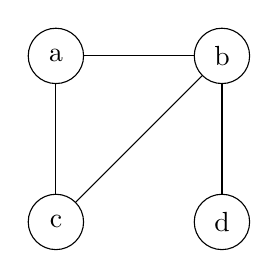
\begin{tikzpicture}
        \tikzstyle{every node}=[draw,circle,minimum size = 2em,node distance = 6em]
        \node (a) {a};
        \node [right of = a] (b) {b} edge(a);
        \node [below of = a] (c) {c} edge(a) edge(b);
        \node [below of = b] {d} edge(b);
    \end{tikzpicture}
\end{figure}

The adjacency matrix and adjacency list for \cref{example_graph} would be:
\begin{table}[ht!]
\begin{minipage}[b]{0.56\linewidth}
\centering
    \begin{tabular}{l|llll}
        & A & B & C & D \\ \hline
         A & 0  & 1  & 1  & 0  \\
         B & 1  & 0  & 1  & 1  \\
         C & 1  & 1  & 0  & 0  \\
         D & 0  & 1  & 0  & 0  \\
    \end{tabular}
    \caption{Adjacency Matrix}
    \label{table:student}
\end{minipage}\hfill
\begin{minipage}[b]{0.4\linewidth}
\centering
\begin{tikzpicture}
    \matrix (M) [matrix of nodes,
                column sep=-\pgflinewidth,
                row sep=0pt,
                nodes in empty cells,
                nodes={draw,fill=gray!20,minimum width=.5cm,outer sep=0pt,minimum height=.7cm,anchor=center},
                column 1/.style={minimum height=.8cm, minimum width=2em}]{
        a &[8mm] b & \mbox{} &[4mm] c & /       \\
        b & a      & \mbox{} & c      & \mbox{}  & [4mm]d    & /  \\
        c & a      & \mbox{} & b      & /         \\
        d & b      & \mbox{} & /      & \mbox{}  \\
    };
    \foreach \i in {1,2,3,4}{
        \path (M-\i-1) [late options={label=left:\i}];
        \draw[->] (M-\i-1.east)--(M-\i-2.west);
        \draw[->] (M-\i-3.center)--(M-\i-4.west);
    }
    \draw[->] (M-2-5.center)--(M-2-6.west);
\end{tikzpicture}
\captionof{figure}{Adjacency List}
\label{fig:image}
\end{minipage}
\end{table}

The running time for these two data structures are shown in
\cref{table:running_time_of_amaj}.

\begin{table}[H]
    \caption{Running Time Analysis for Adjacency Matrix and Adjacency List}
    \label{table:running_time_of_amaj}
    \centering
    \begin{tabular}{l|c|c}
        \hline
        Time & Adjacency Matrix & Adjacency List \\\hline
        visit neighbor & \bigO{1} & \bigO{1}\\
        visit all neighbors & \bigO{n} & \bigO{degree(v)} \\
        test if $uv \in E$ & \bigO{1} & \tikzmark{runanaadaj1}{\bigO{degree(v)}}\\
        add/delete edge & \bigO{1} & \tikzmark{runanaadaj2}{\bigO{n}}\\
        size & \bigO{mn} & \bigO{m+n}
    \end{tabular}
    \begin{tikzpicture}[remember picture,overlay,node distance = 1cm]
        \node[below right = 4em and 1em of runanaadaj1] (notes) {\bigO{1} with hashing.};
        \draw[->,thick] (runanaadaj1.east) to [in=90,out=0] (notes.north);
        \draw[->,thick] (runanaadaj2.east) to [in=90,out=0] (notes.north);
    \end{tikzpicture}
\end{table}


\subsection{Traversing Graph}
\subsubsection{Intuitive Approach}
Assume $G$ is a connected, undirected graph.
Suppose we want to visit every vertex in $G$,
we can use Depth First Search (DFS) is a recursive
manner, as shown in \cref{algo:recursiveDFS}.

\begin{algorithm}[H]
    \caption{Recursive Depth First Search Algorithm}\label{algo:recursiveDFS}
    \begin{algorithmic}[1]
        \Procedure{RecursiveDFS}{$v$}
            \If{$v$ unmarked}
                \State Mark $v$\Comment{has $v$ been visited.}
                \For{each edge $vw$.}
                    \State\ProcedureName{RecursiveDFS}{w}
                \EndFor
            \EndIf
        \EndProcedure
    \end{algorithmic}
\end{algorithm}

Initially, call \ProcedureName{RecursiveDFS}{s},
where $s \in V$ is some start vertex.

Note that the functions was called recursively, forming an implicit stack.
We can re-write as an iteration using an explicit stack,
as shown in \cref{algo:iterativeDFS}.

\begin{algorithm}[H]
    \caption{Iterative Depth First Search Algorithm}\label{algo:iterativeDFS}
    \begin{algorithmic}[1]
        \Procedure{IterativeDFS}{$s$}
            \State\ProcedureName{Push}{s}
            \While{stack not empty}
                \State $s = \ProcedureName{Pop}{}$
                \If{$v$ is unmarked.}
                    \State Mark $v$
                    \For{each edge $vw$}
                        \If{$w$ is unmarked}
                            \Comment{This \emph{if} is optional in some cases.}
                            \State\ProcedureName{Push}{w}
                        \EndIf
                    \EndFor
                \EndIf
            \EndWhile
        \EndProcedure
    \end{algorithmic}
\end{algorithm}

\observation
Traversal algorithms store candidate vertices in a ``bag'',
which can be any structure allowing insertion/deletion.

\subsubsection{Generic Traverse Algorithm}

So we can define this generic traverse algorithm
as shown in \cref{algo:genericTraverse}.


\begin{algorithm}[H]
    \caption{Generic Traverse Algorithm}\label{algo:genericTraverse}
    \begin{algorithmic}[1]
        \Procedure{Traverse}{$s$}
            \State Put $s$ in bag
            \While{bag is not empty}
            \State \tikzmark{algogenericTraverseambiguousPoint}{Take $v$ from bag.}
                \If{$v$ is unmarked}
                    \State Mark $v$
                    \For{each edge $vw$}
                        \If{$w$ is unmarked}
                        \Comment{\tikzmark{algogenericTraverseNote}{This \emph{if} is optional in some cases.}}
                            \State Put $w$ in bag.
                        \EndIf
                    \EndFor
                \EndIf
            \EndWhile
        \EndProcedure
    \end{algorithmic}
    \begin{tikzpicture}[remember picture,overlay,node distance = 1cm]
        \node[above right = 0em and 8em of algogenericTraverseambiguousPoint] (notes)
            {\textbf{This step is ambiguous.}};
        \draw[blue,->,thick] (algogenericTraverseambiguousPoint.east) to [in=180,out=0] (notes.west);
        \node[below = 3em of algogenericTraverseNote, text width=8cm] (notes1)
            {In other application, this line may bot be needed, as for traversing, it is needed.};
        \draw[blue,->,thick] (algogenericTraverseNote) to (notes1);
    \end{tikzpicture}
\end{algorithm}

\observation This traverse algorithm clearly marks each vertex at most once.
Now we want to prove it marks each vertex at least once,
i.e. ``visit'' every vertex. To do this, we can remember each vertex's
parent in the process. The modified algorithm is shown in \cref{algo:genericTraverseM}


\begin{algorithm}[H]
    \caption{Remember Parent version of Generic Traverse Algorithm}\label{algo:genericTraverseM}
    \begin{algorithmic}[1]
        \Procedure{Traverse}{$s$}
            \State Put $(\emptyset,s)$ in bag
            \While{bag is not empty}
                \State Take $(p,v)$ from bag
                    \Comment{\bigO{1} per round.}
                \If{$v$ is unmarked}
                \Comment{\bigO{m} overall, regardless of inner \emph{for}}
                    \State Mark $v$
                    \State $Parent(v) = p$
                    \For{each edge $vw$}
                            \Comment{\bigO{m} overall.}
                        \If{$w$ is unmarked}
                            \State Put $(v,w)$ in bag
                        \EndIf
                    \EndFor
                \EndIf
            \EndWhile
        \EndProcedure
    \end{algorithmic}
\end{algorithm}

\begin{lemma}
    \ProcedureName{Traverse}{s} marks every vertex in connected graph exactly once.

    Set of pair $(parent(v),v)$ with $parent \neq \emptyset$ defines spanning tree.
\end{lemma}

\begin{proof}
    $s$ is marked, so let $v \neq s$.

    Let $(s,\ldots,u,v)$ be shortest path from $s$ to $v$, use induction on path length.
    By induction, $u$ is visited, which implies that when $u$ is marked,
    $(u,v)$ is put in the bag.

    Call a pair $(parent(v),v)$, s.t. $parent(v) \neq \emptyset$ a parent edge.
    Consider the path $(v,parent(v),parent(parent(v)),\ldots)$, this path eventually lead to $s$.
    If every vertex has path to $s$, then parent edge define connected spanning graph.
\end{proof}

\vspace{0.1in}\noindent\textbf{Running Time for Generic Traverse Algorithm}

Each vertex marked exactly once. Each edge $(v,w)$ added to bag at most once
by $v$ and at most once by $w$.

Inner loop executed at most \bigO{m} time.
Outer loop \bigO{m} time. In total, \bigO{m} time.

Note that, this running time analysis ignore bag operation
time (consider \bigO{1} for all bag operations). If bag operation
takes $b$ per operation, \bigO{mb} total time is required.

For connected graph, $n = \bigO{m}$.

\subsubsection{Usage of Using Generic Travers Algorithm}
\begin{enumerate}
    \item Bag is stack $\Longrightarrow$ DFS (results in a long skinny tree).
    \item Bag is queue $\Longrightarrow$ BFS (results in a short fat tree).
    \item If edges have weight, and bag is min priority queue on edge weights.\\
        $\Longrightarrow$ MST, Prim's Algorithm.
    \item Bag is min priority queue on vertex distance.\\
        $\Longrightarrow$ Dijkstra's Algorithm, shortest path tree.
\end{enumerate}

If $G$ is disconnected, we can use a wrap functions to traverse,
as shown in \cref{algo:wrapperGenericTraverse}.

\begin{algorithm}[H]
    \caption{Wrapper for Traverse}\label{algo:wrapperGenericTraverse}
    \begin{algorithmic}[1]
        \Procedure{TraverseAll}{}
            \For{all vertices $v$}
                \If{$v$ is unmarked}
                    \State\ProcedureName{Traverse}{v}
                \EndIf
            \EndFor
        \EndProcedure
    \end{algorithmic}
\end{algorithm}

\begin{lemma}
    \ProcedureName{TraverseAll}{} marks every vertex in disconnected graph exactly once.

    Set of pair $(parent(v),v)$ with $parent \neq \emptyset$ defines spanning forest.
\end{lemma}

\subsection{Standard Graph Algorithm}
\begin{enumerate}[label=Step {\arabic*}, leftmargin=0.5in]
    \item Maintain set $S$ of visited vertices, and $T \setminus S$ of unvisited.
    \item Maintain tree over $S$.
    \item Repeat:
        \begin{enumerate}
            \item Pick vertex $w$ in $T$, which is adjacent to $S$.
            \item Add to $S$, remove from $T$, update tree on $S$.
        \end{enumerate}
\end{enumerate}

\subsection{Depth First Search}
\subsubsection{Formal Definition}
The Formal definition of DFS is shown in \cref{algo:formalDFS}.
\begin{algorithm}[H]
    \caption{Formal Definition of DFS}\label{algo:formalDFS}
    \begin{algorithmic}[1]
        \Procedure{DFS}{$v$}
            \State Mark $v$
            \For{each edge $vw$}
                \If{$w$ is unmarked}
                    \State\ProcedureName{DFS}{w}
                \EndIf
            \EndFor
        \EndProcedure
    \end{algorithmic}
\end{algorithm}

\observation The procedure create a similar stack of that
in \cref{algo:genericTraverse}, but it's the program's stack.
When \ProcedureName{DFS}{w} makes recursive call, it stores
current program on program stack, i.e. when \ProcedureName{DFS}{v}
calls \ProcedureName{DFS}{w}, \ProcedureName{DFS}{v} is on stack.


Given $v$ in undirected $G$, \ProcedureName{DFS}{v} visits
all vertices in $v$'s component.

\begin{algorithm}[H]
    \caption{DFS All the Component}\label{algo:dfsall}
    \begin{algorithmic}[1]
        \Procedure{DFSAll}{$G$}
            \For{all $v \in V$}
                \If{$v$ is unmarked}
                    \State\ProcedureName{DFS}{v}
                \EndIf
            \EndFor
        \EndProcedure
    \end{algorithmic}
\end{algorithm}

\subsubsection{Count and Label Components}
DFS Algorithm can be modified to count and label all the components.
\begin{algorithm}[H]
\caption{Count and Label the Components}\label{algo:countlabel}
    \begin{algorithmic}[1]
        \Procedure{CountAndLabel}{$G$}
            \State $count = 0$
            \For{all $v \in V$}
                \If{$v$ is unmarked.}
                    \State $count = count + 1$
                    \State\ProcedureName{LabelComponent}{v,count}
                \EndIf
            \EndFor
            \Return $count$
        \EndProcedure
        \Procedure{LabelComponent}{$v,count$}
            \State Mark $v$
            \State $component(v) = count$
            \For{each $vw$}
                \If{$w$ is unmarked}
                    \State\ProcedureName{LabelComponent}{w,count}
                \EndIf
            \EndFor
        \EndProcedure
    \end{algorithmic}
\end{algorithm}

\subsubsection{Pre/Post Order Traverse of Binary Tree}

Originally, the definition are:
\begin{itemize}
    \item Pre-order: visit, recursive call on left, recursive call on right.
    \item Post-order: recursive call on left, recursive call on right, visit.
\end{itemize}

Consider the problem in the view of DFS:
\begin{itemize}
    \item Pre-order: vertices put on stack;
    \item Post-order: vertices taken off from stack.
\end{itemize}

A modified algorithm is shown in \cref{algo:DFSprepost}
\begin{algorithm}[H]
    \caption{Pre/Post Order Based on DFS}\label{algo:DFSprepost}
    \begin{algorithmic}[1]
        \Procedure{DFSAll}{$G$}
            \State $clock = 0$
            \For{all $v \in V$}
                \If{$v$ is unmarked}
                    \State\ProcedureName{DFS}{v}
                \EndIf
            \EndFor
        \EndProcedure
        \Procedure{DFS}{$v$}
            \State Mark $v$
            \State \ProcedureName{Previsit}{v}
            \For{each edge $vw$}
                \If{$w$ is unmarked}
                    \State\ProcedureName{PreVisit}{w}
                \EndIf
            \EndFor
            \State\ProcedureName{PostVisit}{v}
        \EndProcedure
        \Procedure{PreVisit}{$v$}
            \State $pre(v) = clock$
            \State $clock = clock + 1$
        \EndProcedure
        \Procedure{PostVisit}{$v$}
            \State $post(v) = clock$
            \State $clock = clock - 1$
        \EndProcedure
    \end{algorithmic}
\end{algorithm}

\subsubsection{Directed Graphs and Reachability}
\begin{itemize}
    \item For undirected graph, \ProcedureName{DFS}{v} explores the component of $v$.
    \item For directed graph, it is trickier.
        \begin{itemize}
            \item For $v,u$ in directed graph, $u$ is reachable from $v$,
                if directed path from $v$ to $u$.
            \item Let \ProcedureName{Reach}{v} be set of vertices
                reachable from $v$.
            \item If $v \in \ProcedureName{Reach}{v}$, $v$ may or may not be in
                \ProcedureName{Reach}{u}.
        \end{itemize}
\end{itemize}


\subsection{Directed Acyclic Graphs}
\subsubsection{Definition of DAG}
A \textbf{DAG} is a directed graph with no directed cycles.
\begin{itemize}
    \item For a DAG, if $u \in \ProcedureName{Reach}{v}$,
        then $v \notin \ProcedureName{Reach}{u}$.
    \item A source is a vertex with no incoming edges.
    \item A sink is a vertex with no outgoing edges.
    \item Every DAG has at least one source and at least one sink.
    \item Checking if graph is a DAG need \bigO{n+m} time using DFS.
\end{itemize}
To make concept simpler:
\begin{itemize}
    \item Let $G$ be a directed graph.
    \item $G^\prime$ obtained by adding source $s$, a directed edge from
        $s$ to all vertices of $G$.
    \item $G$ is a DAG $\iff$ $G^\prime$ is a DAG (if and only if).
\end{itemize}

\subsubsection{Algorithm to Determine a DAG}
To illustrate is a program manner,consider 3 status during the traversal.
\begin{itemize}
    \item \textsc{New}: never been of program stack;
    \item \textsc{Active}: is currently on the stack;
    \item \textsc{Done}: is off stack, but was previously on.
\end{itemize}
Thus, the DFS algorithm can be modified as shown in \cref{algo:acyclicDFS}

\begin{algorithm}[H]
    \caption{Determine Whether a Graph is DAG}\label{algo:acyclicDFS}
    \begin{algorithmic}[1]
        \Procedure{IsAcyclic}{$G$}
            \State Add vertex $s$
            \For{all $v \neq s$ in $V$}
                \State Add edge $s \rightarrow v$
                \State \ProcedureName{Status}{v} = \textsc{New}
            \EndFor
            \Return \ProcedureName{IsAcyclicDFS}{s}
        \EndProcedure
        \Procedure{IsAcyclicDFS}{$v$}
            \State \ProcedureName{Status}{v} = \textsc{Active}
            \For{each edge $v \rightarrow w$}
                \If{\ProcedureName{Status}{w} = \textsc{Active}}
                    \Return False
                \ElsIf{\ProcedureName{Status}{w} = \textsc{New}}
                    \If{\ProcedureName{IsAcyclicDFS}{w} = False}
                        \Return False
                    \EndIf
                \EndIf
            \EndFor
            \State \ProcedureName{Status}{v} = \textsc{Done}
            \Return True
        \EndProcedure
    \end{algorithmic}
\end{algorithm}

\subsubsection{Proof of Correctness}

Prove ``False'' implies cycle.

Suppose ``False'' is returned, then find edge $v \rightarrow w$,
s.t. \ProcedureName{Status}{w} = \textsc{Active}.
\begin{itemize}
    \item If $w$ is \textsc{Active}, then it's on the stack and
        $v$ is currently on top of stack.
    \item If vertex $b$ directly on top of $c$ on stack,
        then there must be an edge $c \rightarrow b$.
    \item Thus there must be a direct path $w \rightarrow \ldots \rightarrow v$,
        appending $v \rightarrow w$ gives a cycle.
\end{itemize}

\noindent Prove cycle leads to ``False''.

Let $w$ be first vertex in cycle that we visit,
$v$ is vertex before $w$ in cycle. Then, there exist a path
$w \rightarrow \ldots \rightarrow v \rightarrow w$.

Since $w$ visited first. \ProcedureName{IsAcyclicDFS}{w}
called first in the cycle.

There is a directed path from $w$ to $v$, so \ProcedureName{IsAcyclicDFS}{v}
is called while $w$ on stack.
During \ProcedureName{IsAcyclicDFS}{v}, $v \rightarrow w$ is looked at.
Thus, result in False.


\subsection{Topological Sort}
Given directed $G$, topological ordering is a total order $\prec$
on the vertices s.t. $u \prec v$ for every edge $u \rightarrow v$.

Informally, a topological sort is the order arranges vertices from
left to right, s.t. all edges go from left to right.
An example is shown in \cref{fig:topoexample}
\begin{figure}[H]
    \caption{Example for Topological Sort}\label{fig:topoexample}
    \centering
    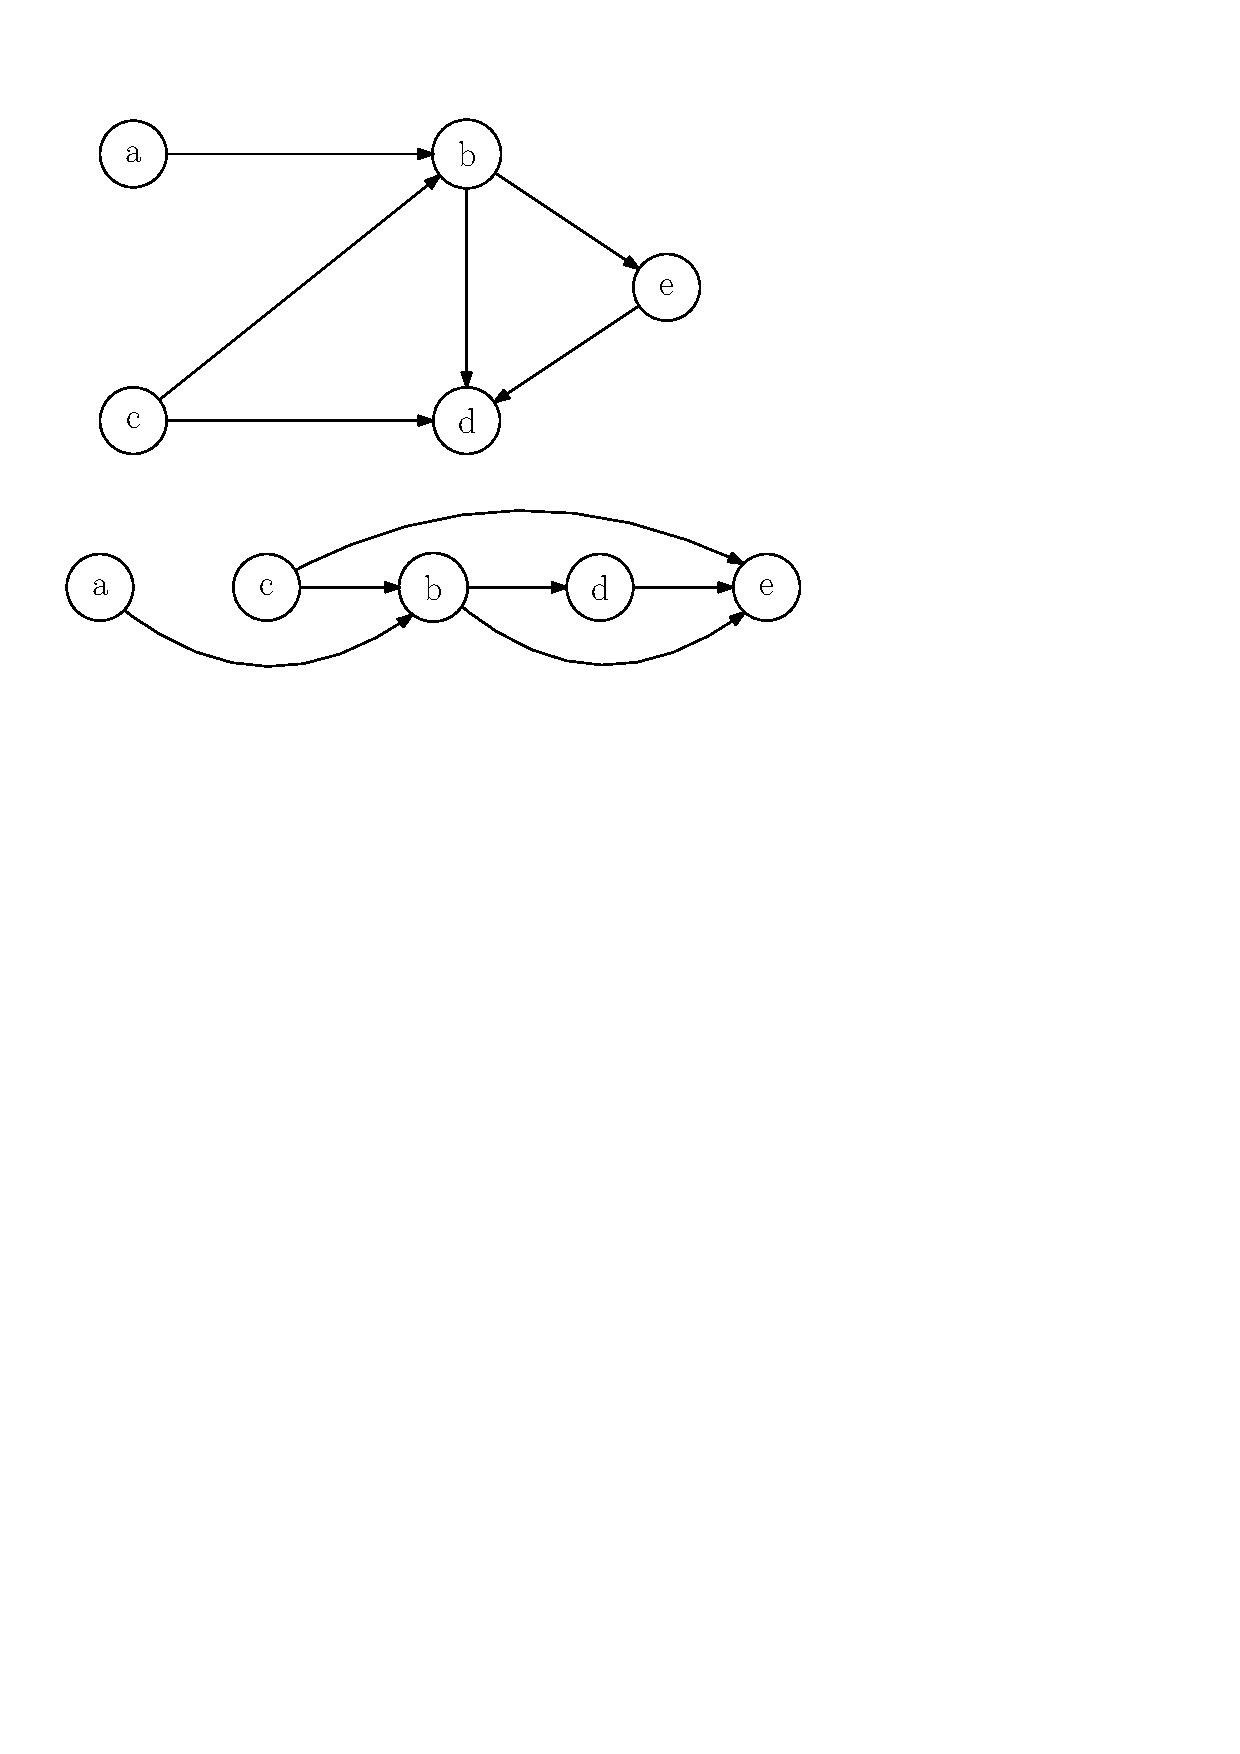
\includegraphics[scale=0.8]{fig/topo1.pdf}
\end{figure}

\observation

The most important fact:
\begin{quote}
$G$ has a topological ordering if and only if no cycles exist,
i.e. $G$ is a DAG.
\end{quote}

A DAG has at least one source/sink, thus the topological sort has
two implementation, one starts from sink, the other starts from source.
The algorithm is shown in \cref{algo:toposink} and \cref{algo:toposource}.

\begin{minipage}[t]{0.48\linewidth}
\vspace{0pt}
\begin{algorithm}[H]
    \caption{Topo-Sort from Source}\label{algo:toposource}
    \begin{algorithmic}[1]
        \Procedure{TopologicalSort}{$G$}
            \State $n = |V|$
            \For{$i = 1 \text{ to } n$}
                \State $v = \text{ any Source }$
                \State $S[i] = v$
                \State Delete $v$
            \EndFor
            \Return $S[1 \ldots n]$
        \EndProcedure
    \end{algorithmic}
\end{algorithm}
\vspace{2pt}
\end{minipage}\hfill
\begin{minipage}[t]{0.48\linewidth}
\vspace{0pt}
\begin{algorithm}[H]
    \caption{Topo-Sort from Sink}\label{algo:toposink}
    \begin{algorithmic}[1]
        \Procedure{TopologicalSort}{$G$}
            \State $n = |V|$
            \For{$i = n \text{ to } 1$}
                \State $v = \text{ any Sink}$
                \State $S[i] = v$
                \State Delete $v$
            \EndFor
            \Return $S[1 \ldots n]$
        \EndProcedure
    \end{algorithmic}
\end{algorithm}
\vspace{2pt}
\end{minipage}

In the algorithm, $v = \text{ any Sink/Source}$ is ambiguous.
Naively, the algorithm takes \bigO{nm} time.

\begin{lemma}
    For any DAG, first vertex marked \textsc{Done} by
    \ProcedureName{IsAcyclic}{} is a sink.
\end{lemma}
\begin{proof}
    Let $v$ be first vertex marked \textsc{Done}. Suppose $v \rightarrow w$ exists.
    \begin{itemize}
        \item If $w$ marked \textsc{Done}, results in contradiction.
        \item If $w$ marked \textsc{Active}, then there is a cycle.
        \item If $w$ marked \textsc{New}, then recursively call on $w$.
            Thus $w$ marked \textsc{Done} before $v$.
    \end{itemize}
    In all three cases, $v$ must be a sink.
\end{proof}

\observation
\begin{itemize}
    \item \ProcedureName{IsAcyclic}{$G$} is modified DFS.
    \item First vertex marked \textsc{Done} is first off stack.
    \item First off stack is the first post order.
    \item This behavior repeats.
\end{itemize}
Thus, Topological order is reverse post order traverse.

Topological ordering computed in \bigO{n+m} time with DFS.

Why does linear time matter?
\begin{itemize}[label={-}]
    \item Scheduling: two jobs $a \rightarrow b$ means
        $a$ depends on $b$.\\
        Reverse topological order is valid job scheduling.
    \item Dynamic Programming.\\
        Recursive sub-problem is a vertex, edges to other sub-problems
        you depend on.
\end{itemize}

\subsection{Strong Connectivity}
$u$ and $v$ are in same strong component if $u \in \ProcedureName{Reach}{v}$
and $v \in \ProcedureName{Reach}{u}$.

Strong Component defines an eequivalent relation.
\begin{itemize}
    \item If $u,v$ in some SC, and $v,w$ in some SC, then
        $u,w$ in same SC.
    \item Define a vertex partition: given two strong components
        $S_1$, $S_2$, $S_1 \cap S_2 = \emptyset$,
        and every vertex in same SC.
\end{itemize}

Denote \ProcedureName{SSC}{G} as Strong Connected Component Graph,
obtained by collapsing each component to vertex, each edge
from $S_1$ to $S_2$, if and only if $\exists u \in S_1, v \in S_2$
s.t. $u \rightarrow v$ in $G$.

\ProcedureName{SSC}{G} is DAG.
In a DAG, every vertex is its own SC.

To compute \ProcedureName{SSC}{G}, call a component sink if sink in
\ProcedureName{SSC}{G}.
Observe that for sink components, \ProcedureName{DFS}{v} for $v \in S$
explores all vertices in $S$.
Thus, the algorithm can be defined as \cref{algo:computeSSC}.

\begin{algorithm}[H]
    \caption{Algorithm to Compute Strong Components}\label{algo:computeSSC}
    \begin{algorithmic}[1]
        \Procedure{StrongComponents}{$G$}
            \State $count = 0$
            \While{$G$ is not empty}
                \State $count = count + 1$
                \State $v = $ any vertex in sink component.
                \State $c = \ProcedureName{DFSLabel}{v,count}$
                \State Remove $c$ from $G$.
            \EndWhile
        \EndProcedure
    \end{algorithmic}
\end{algorithm}

\subsection{Minimum Spanning Tree ( MST )}

\subsubsection{MST Definition}
\AlgoInput Undirected, weighted, connected graph $G$.
Assume there is a function $w:E \rightarrow R$

\AlgoOutput Find the minimum spanning tree of $G$,
i.e. the spanning tree $T$ which minmimizes
$\displaystyle w(T) = \sum_{e \in T} w(e)$.

\subsubsection{MST Property}
Why use MST?

If vertices represent nodes in a network,
and weights represent connection cost.
MST is cheapest way to connect all nodes.

A example of MST is shown in \cref{fig:MSTexample}.
\begin{figure}[ht]
    \caption{Example for MST}\label{fig:MSTexample}
    \centering
    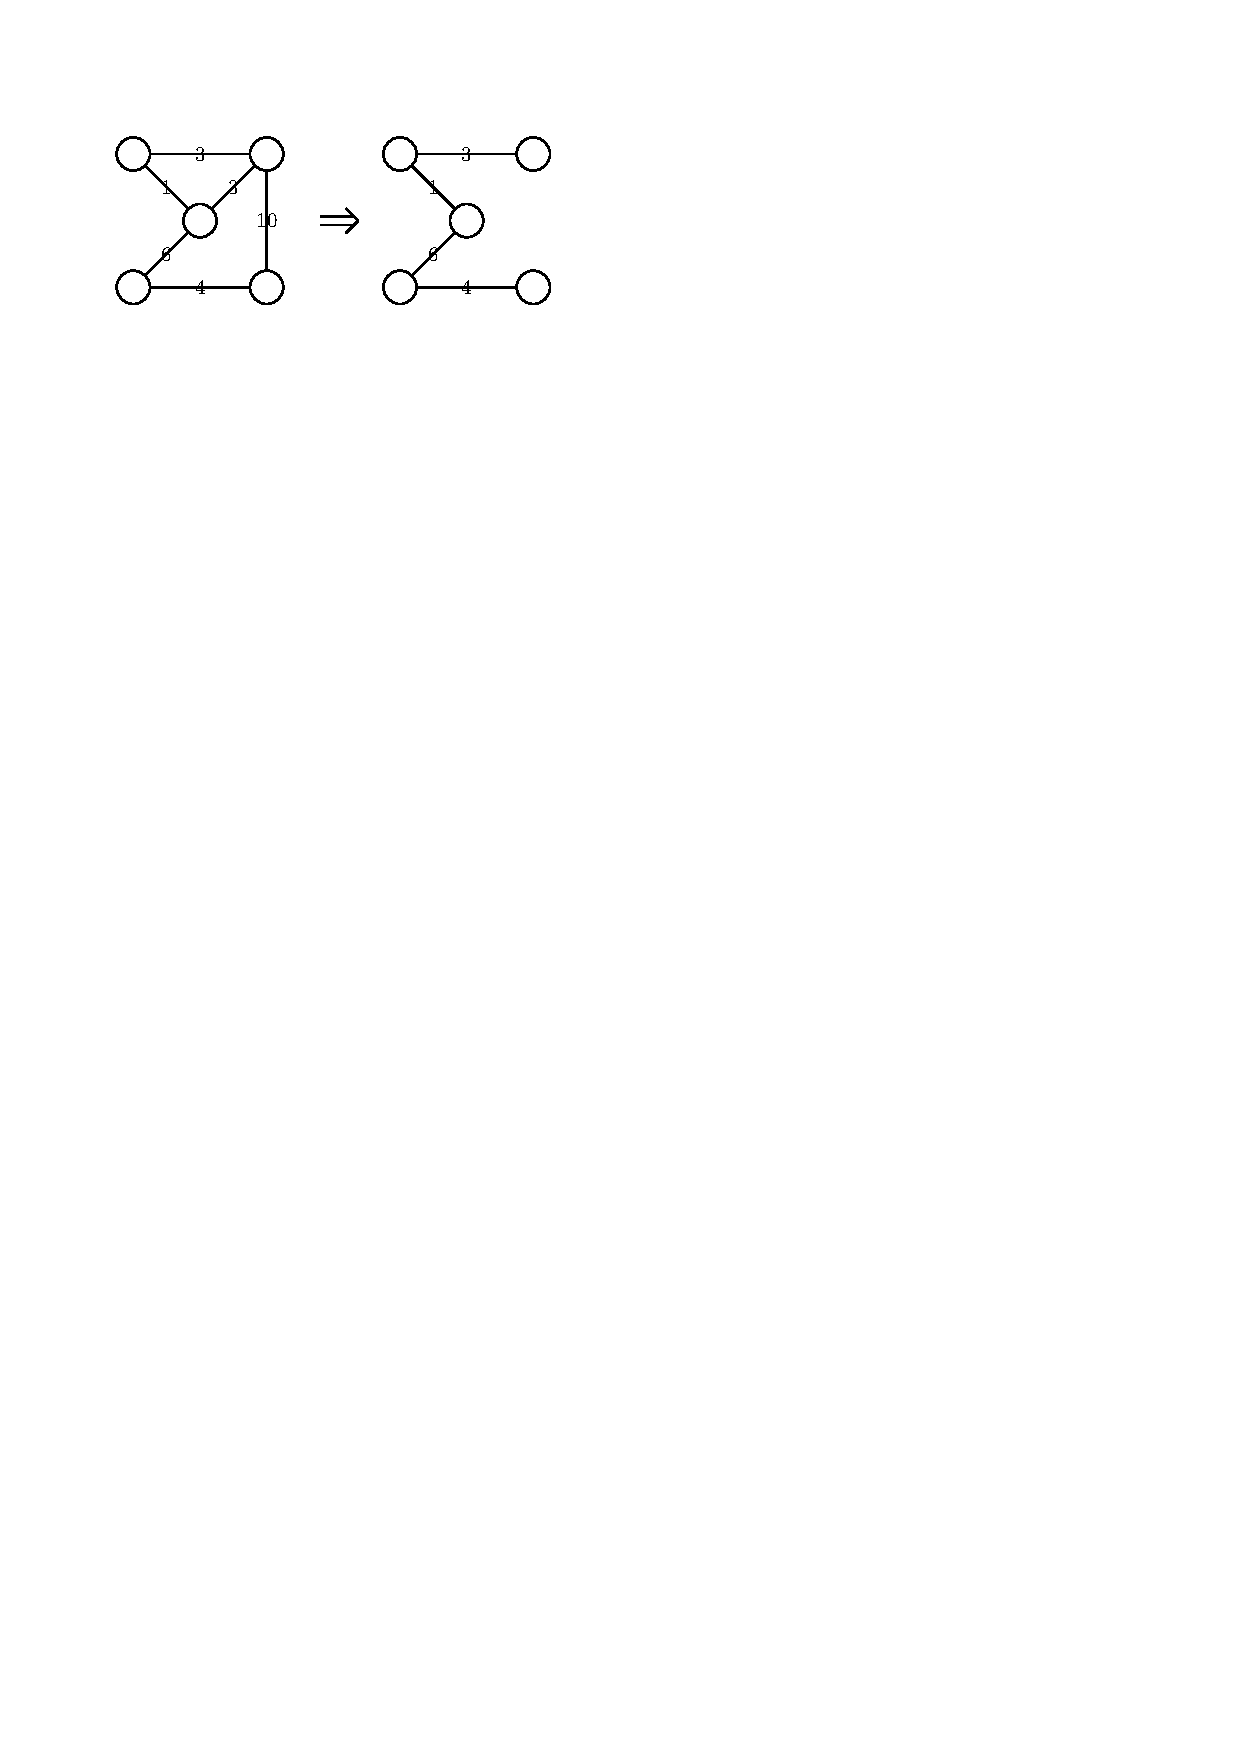
\includegraphics[scale=1.2]{fig/MSTexample}
\end{figure}

\observation

Some properties are obvious:
\begin{itemize}
    \item If all weights distinct, can prove MST is unique.
    \item If all weights equal, any spanning tree is a MST.
\end{itemize}

\noindent \textbf{Main MST Property}

A partition of $V$ is a pair $S,R \subseteq V$,
s.t. $S \cap R = \emptyset$ and $S \cup R = V$.
Given a partition $S,R \subseteq V$, \ProcedureName{mwe}{S,R}
denotes minimum weight edge $u\rightarrow v$, s.t. $u \in S$, $v \in R$.
\begin{itemize}
    \item For any partition $S,R$, $\ProcedureName{mwe}{S,R} \in MST$.
    \item If $e$ is not minimum weight edge of any partition,
        then $e \notin \ProcedureName{MST}{G}$.
\end{itemize}

\begin{proof}
    First, prove that for any partition $S,R$, $\ProcedureName{mwe}{S,R} \in MST$.

    Let $S,R$ be a partition and let $e = \ProcedureName{mwe}{S,R}$.

    Suppose $e = u \rightarrow v$, where $u \in S$, $v \in R$.
    Consider any spanning tree $T$, which does not contain $e$.
    $T$ contains unique path from $u$ to $v$.
    Some edges in this path has endpoint in $S$ and another in $R$.
    Let $e^\prime$ be such an edge.

    Remove $e^\prime$ from $T$, gives a spanning forest, with two trees.
    $u$ and $v$ must be in different trees.

    Hence adding $e$ connects two trees, producing single spanning tree
    $T^\prime = T - e^\prime + e$. $weight(e) < weight(e^\prime)$, so $weight(T^\prime) < weight(T)$.
    $T$ is not MST, result in contradiction.

    Then, prove that if $e$ is not minimum weight edge of some partition,
    then it's not in MST.

    Let $T$ be the MST.
    Consider any edge $e^\prime \in T$. $e^\prime$ define partition of $V$.

    Just proved minimum weight edge across this partition must be in MST.
    Since $e^\prime$ is the only edge in $T$ crossing this partition,
    it must be min weight.
\end{proof}

\subsubsection{MST Algorithm ( General )}
General idea of MST algorithm is:
\begin{quote}
Maintain a spanning forest, initially is $n$ isolated vertices.
Add an edge of MST, update forest, and repeat.
\end{quote}
All the algorithm follows is the variation of this general idea.

\subsubsection{Prim's Algorithm}
\vspace{0.1in}\noindent\textbf{Key point}
\begin{itemize}
    \item Pick vertex $s$. Grow MST from $s$, call it $T$.
    \item In each round, find the edge
        $e = \ProcedureName{mwe}{T, V \setminus T}$.
        Add $e$ to $T$ and repeat.
    \item To find $e$, store edges adjacent to $T$
        in min priority queue.
\end{itemize}
The algorithm is shown in \cref{algo:prim}
\begin{algorithm}[H]
    \caption{Prim's Algorithm}\label{algo:prim}
    \begin{algorithmic}[1]
        \Procedure{Prim}{$s$}
            \State Initial an empty minimum priority queue $Q$
            \State Mark $s$
            \For{all edges $s \rightarrow w$}
                \State Put $(s,w)$ in $Q$
            \EndFor
            \While{$Q$ is not empty}
                \State $(p,v) = Q.pop$
                \If{$v$ is unmarked}
                    \State Mark $v$
                    \State $\ProcedureName{Parent}{v} = p$
                    \For{each edge $v \rightarrow w$}
                        \State Put $(v,w)$ in $Q$
                    \EndFor
                \EndIf
            \EndWhile
        \EndProcedure
    \end{algorithmic}
\end{algorithm}

\observation
This traverse with bag = min queue. Marked mean in tree, not in queue.

An example is shown in \cref{fig:prim}.
\begin{figure}[ht!]
    \caption{Example for MST}\label{fig:prim}
    \centering
    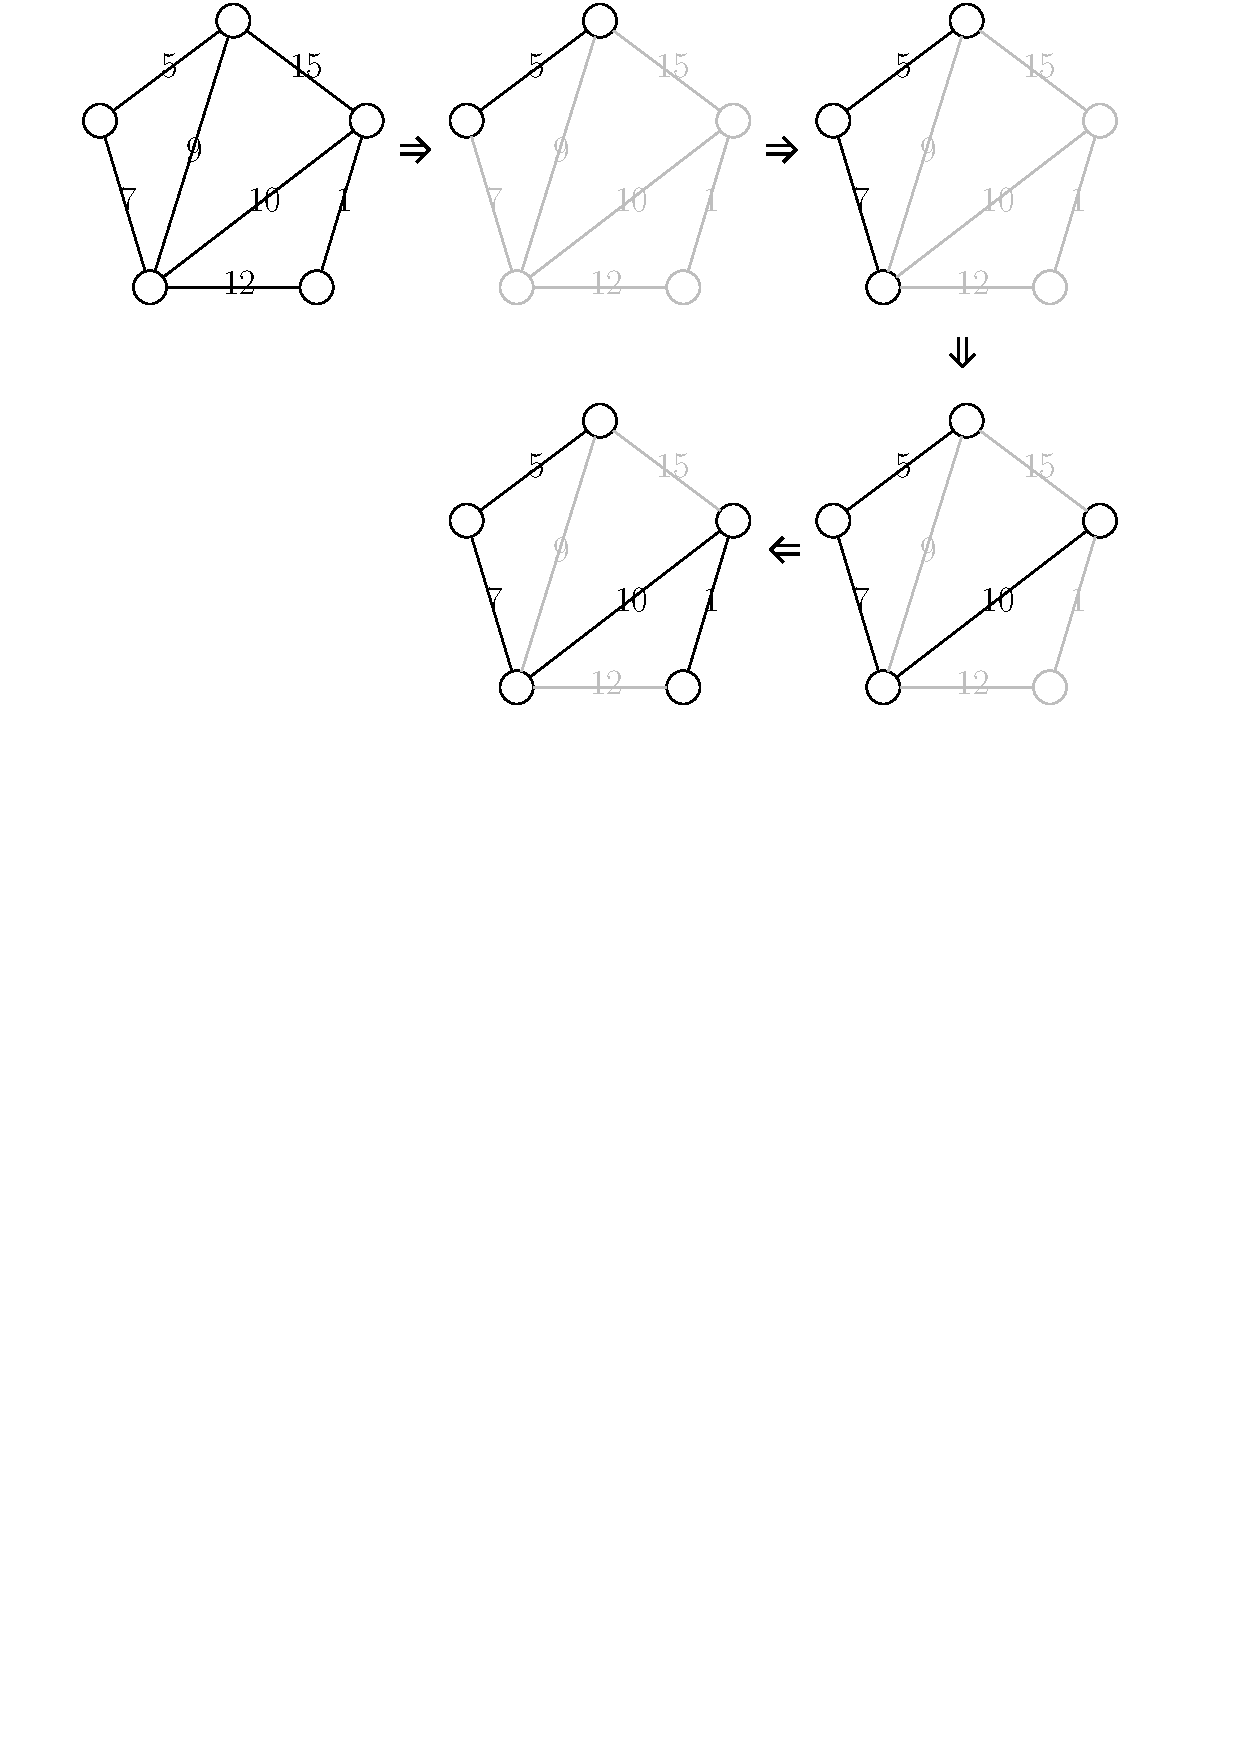
\includegraphics[width=.6\linewidth]{fig/PrimExample}
\end{figure}

\analysis

Each time add \ProcedureName{mwe}{T, V \setminus T},
which we know is in MST, so correct.

Recall that for traverse, running time depend on bag operation cost.
Specifically each edge is added/renewed from $Q$ once,
and this dominates runtime.

If $Q$ implemented in binary min heap, all operations take
\[\bigO{\lg{heap size}} = \bigO{\log(m)} = \bigO{\log(n)}\]
time. Thus total time is \bigO{m \log n}

Note that the running time can be improved to
\bigO{m + n\log n} time using Fibonacci Heap, see Jeff's note.

\subsubsection{Borvka's Algorithm}
\vspace{0.1in}\noindent\textbf{Key point}
\begin{itemize}
    \item Start with forest of singletons, $F = (v,\emptyset)$.
    \item Repeat until $F$ is a single tree:
        For every $T \in F$, add \ProcedureName{mwe}{T, V \setminus T}.
\end{itemize}
The algorithm is shown in \cref{algo:borvka}
\begin{algorithm}[H]
    \caption{Borvka's Algorithm}\label{algo:borvka}
    \begin{algorithmic}[1]
        \Procedure{Borvka}{$V,E$}
            \State $F = (V, \emptyset)$
            \State $count = \ProcedureName{CountAndLabel}{F}$
            \While{$count > 1$}
                \State \ProcedureName{AddAllMWE}{E,F,count}
                \State $count = \ProcedureName{CountAndLabel}{F}$
            \EndWhile
            \Return $F$
        \EndProcedure
        \State
        \Procedure{AddAllMWE}{$E,F,count$}
            \For{$i = 1 \text{ to } count$}
            \State $S[i] = NULL$ \Comment{ $w(null) = \infty$ }
            \EndFor
            \For{each edge $uv \in E$}
                \If{$label(u) \neq label(v)$}
                    \If{$weight(uv) < w(S[label(u)])$}
                        \State $S[label(u)] = uv$
                    \EndIf
                    \If{$weight(uv) < w(S[label(v)])$}
                        \State $S[label(v)] = uv$
                    \EndIf
                \EndIf
            \EndFor
            \For{$i = 1 \text{ to } count$}
                \If{$S[i] \neq NULL$}
                    \State add $S[i]$ to $F$
                \EndIf
            \EndFor
        \EndProcedure
    \end{algorithmic}
\end{algorithm}

$S[i]$ stores minimum weight edge with exactly one endpoint in tree $i$.

\analysis

The algorithm is correct since add \ProcedureName{mwe}{T, V \setminus T}
for each $T \in F$.

The running time:
\begin{itemize}
    \item \ProcedureName{CountAndLabel}{F} takes \bigO{n} time,
        since $F$ has \bigO{n} edge.
    \item \ProcedureName{AddAllMWE}{} takes \bigO{m} time,
        since $\bigO{m + n} = \bigO{m}$.
    \item While-loop takes \bigO{m+n} = \bigO{m} per iteration,
        in total performs \bigO{\lg n} iterations.
\end{itemize}
Thus, total running is \bigO{m\log n}.

\subsubsection{Kruskal's Algorithm}

\vspace{0.1in}\noindent\textbf{Key point}
\begin{itemize}
    \item Sort edges in increasing weight order.
    \item Go through edges in increasing order,
        add edge $e$ if its endpoints in different trees.
\end{itemize}

\vspace{0.1in}\noindent\textbf{Correctness}
1
Suppose we add $e$ joing $T_1,T_2 \in F$,
then $e$ must be \ProcedureName{mwe}{T_1, V \setminus T_1}.
If not, then there was cheaper edge $e^\prime$,
but in which case, $e^\prime$ should be add first.

The difficulty is maintaining $F$.
For Borvka, spend \bigO{m} time to update $F$.
Hence, now consider edges one at a time leads to
\bigO{m \times m} = \bigO{m^2} time.

\vspace{0.1in}\noindent\textbf{Union Find}

Union Find is a data structure which can do the following:
\begin{itemize}
    \item \ProcedureName{MakeSet}{V}: make set (i.e. tree in forest)
        with just $V$.
    \item \ProcedureName{Find}{u}: return set id (some vertex in tree).
    \item \ProcedureName{Union}{u,v}: merges sets containing $u$ and $v$.
\end{itemize}
All operation of Union Find take \bigO{\alpha(n)} time.

The algorithm is shown in \cref{algo:kruskal}

\begin{algorithm}[H]
    \caption{Kruskal's Algorithm}\label{algo:kruskal}
    \begin{algorithmic}[1]
        \Procedure{Kruskal}{$s$}
            \State sort $E$ by increasing weight order
            \State $F = (V, \emptyset)$
            \For{each vertex $v \in V$}
                \ProcedureName{MakeSet}{v}
            \EndFor
            \For{$i = 1 \text{ to }|E|$}
            \State $uv = i\text{th \textbf{heaviest} edge in } E$
                \If{$\ProcedureName{Find}{u} \neq \ProcedureName{Find}{v}$}
                    \State \ProcedureName{Union}{u, v}
                    \State add $uv$ to $F$
                \EndIf
            \EndFor
            \Return $F$
        \EndProcedure
    \end{algorithmic}
\end{algorithm}

\analysis

The running time:
\begin{itemize}
    \item \bigO{m} find operations.
    \item \bigO{n} union operations.
    \item \bigO{n} makeset operations.
\end{itemize}
So other than sorting, total time is \bigO{m\alpha(n)}.

Sorting takes \bigO{m\log m} = \bigO{m \log n} time,
dominating the total running.

Thus, total running time would be \bigO{m \log n}.

\subsection{Shortest Paths}
\AlgoInput Weighted directed graph $G$ with labeled
source $s$ and target $t$.

\AlgoOutput Find shortest $s-t$ path, i.e. directed
path $P$ from $s$ to $t$ that minimized
\[w(P) = \sum_{w \rightarrow v \in P}w(u \rightarrow v)\]

Note that we can allow negative weights,
but cannot be negative cycles.

A example of no SP is shown in \cref{fig:spexample}.

\begin{figure}[ht!]
    \caption{Example for No Shortest Path}\label{fig:spexample}
    \centering
    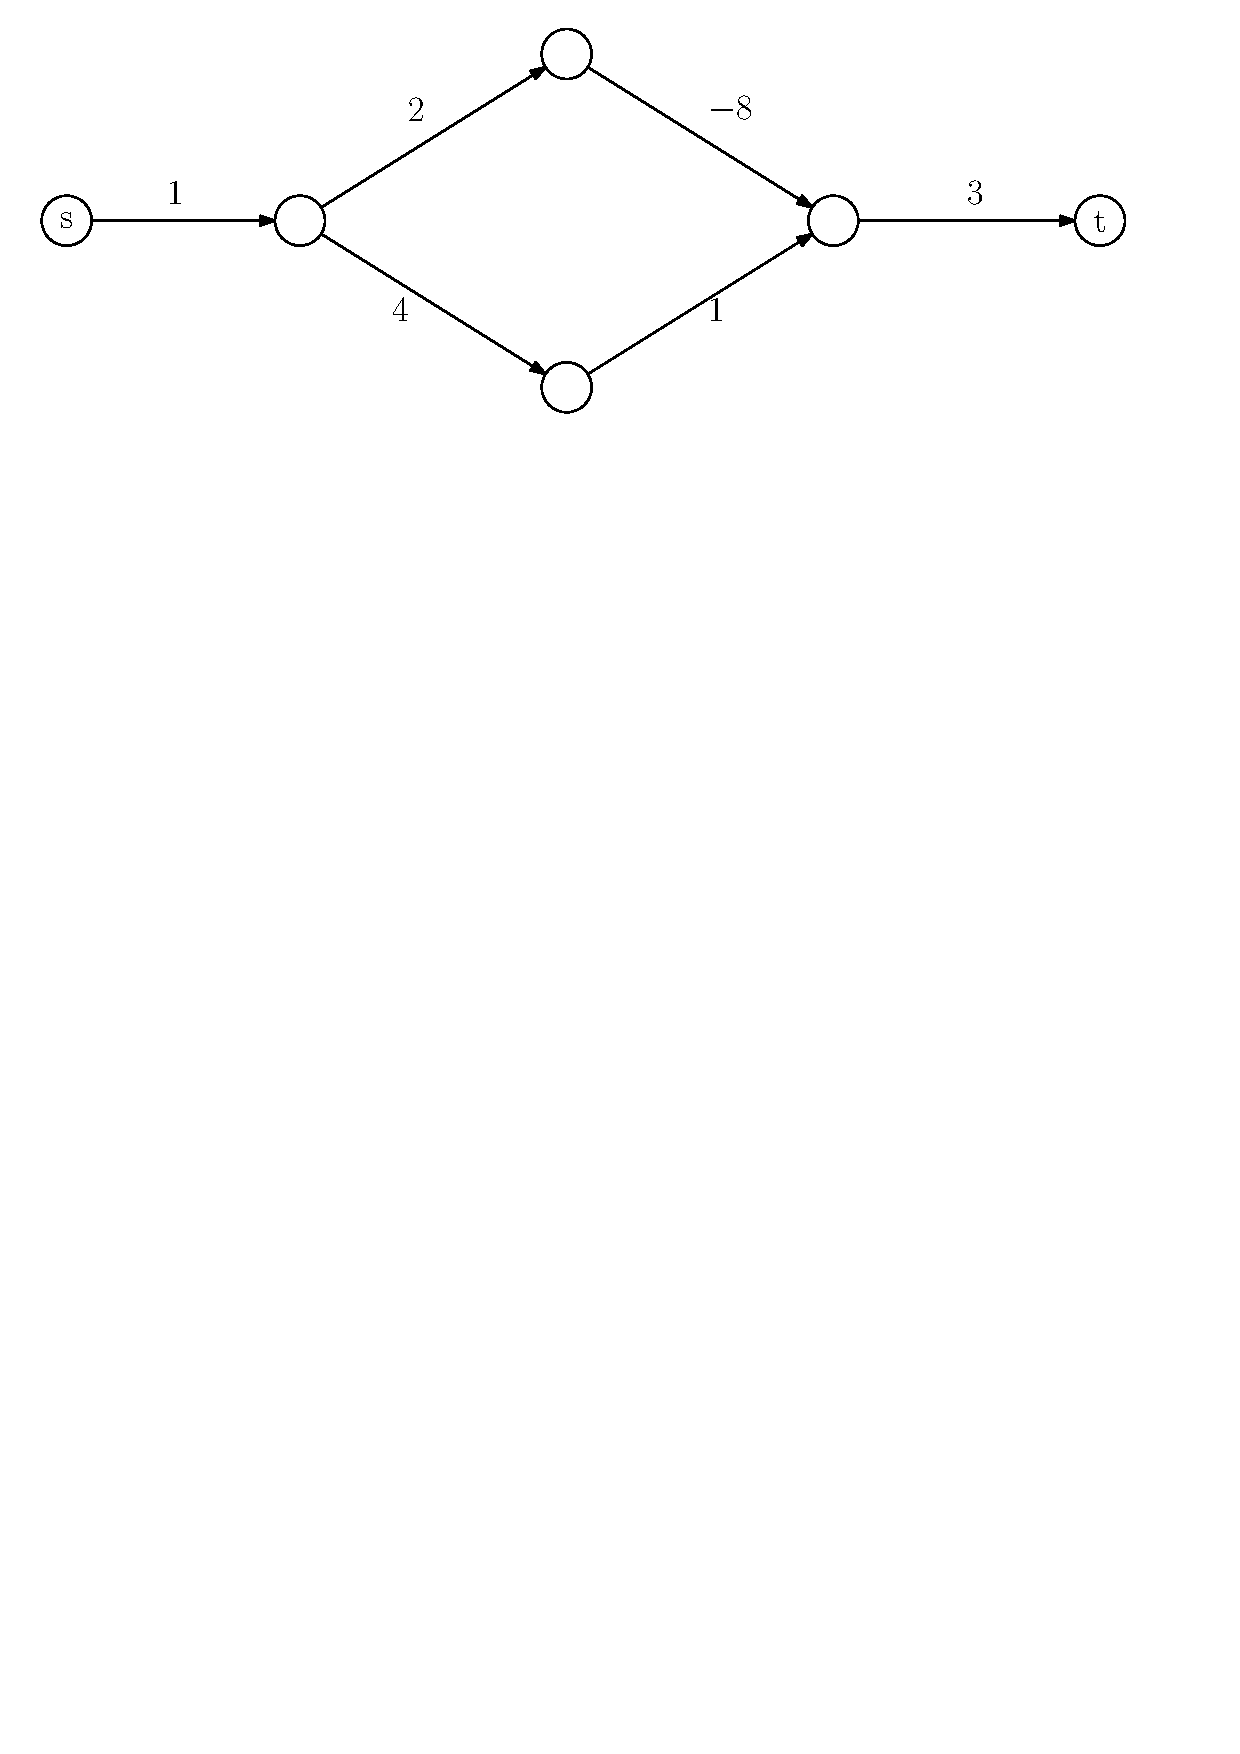
\includegraphics[width=.9\linewidth]{fig/spExample}
\end{figure}

\subsubsection{Single Source Shortest Path ( SSSP )}
Almost every algorithm to find shortest $s-t$ path find
shortest path to every vertex. 
We can represent all shortest paths from $s$ using
a spanning tree rooted at $s$.

\textbf{Why a tree satisfied?}

Suppose shortest $s-w$ path passes through $v$
and shortest $s-t$ path passes through $v$.
The subpath of a shortest path is a shortest path.

\subsubsection{SSSP Algorithm}
Most SSSP algorithms have same structure.

For every vertex $v$, store two values.
\begin{itemize}
    \item $dist(v) =$ length of tentative shortest $sv$ path, or $\infty$ if no $s-v$ path exists.
    \item $pred(v) =$ predecessor of $v$ in tentative shortest $s-v$ path tree.
\end{itemize}

Predecessor pointers define tentative shortest path tree.

Initially, we know $dist(s) = 0$, $pred(s) = null$,
and for every $v \neq s$, initially $dist(v) = \infty$, $pred(v) = null$
to indicate we don't know if there is $s-v$ path.

As we run algorithm $dist(v)$ values may decrease,
but always upper bound tree distances.

During algorithm execution, an edge $u \rightarrow v$ is ``tense''
if $dist(v) + w(u \rightarrow v) < dist(v)$.
If $u \rightarrow v$ tense, clearly shortest path from $s$ to $v$ is wrong,
since $s-u$ path followed by $u \rightarrow v$ is shortest.

\subsubsection{Generic SSSP algorithm}
The general idea is:
\begin{quote}
    Repeated find tense edge and relax it.
\end{quote}
The relax operation is defined as \cref{algo:relax}.

\begin{algorithm}[H]
    \caption{Relax Operation in SSSP Algorithm}\label{algo:relax}
    \begin{algorithmic}[1]
        \Procedure{Relax}{$u \rightarrow v$}
            \State $dist(v) = dist(u) + w(u \rightarrow v)$
            \State $pred(v) = u$
        \EndProcedure
    \end{algorithmic}
\end{algorithm}

The algorithm stops when no tense edges. This can prove the following:
\begin{enumerate}[label={\arabic*)}]
    \item $dist(v) \geq \text{ true distance from $s$ to $v$ at all times. }$
    \item Algorithm halts, i.e. at some finite time, no more tense.
    \item When algorithm halts, all $dist(v)$ values correct.
\end{enumerate}

\begin{proof}
    For 1), prove $\forall v \in V$, $dist(v)$ is either $\infty$ or the length of $s-v$ walk.

    Use induction on number of relaxations.
    \begin{itemize}
        \item Consider $v \in V$, if $v$ not updated in previous relax,
            then holds by induction.
        \item If $v$ updated, then $dist(v) = dist(u) + w(u \rightarrow v)$,
            and $dist(u)$ is the length of walk by induction.
    \end{itemize}

    For 2).

    In 1) can actually prove $dist(v)$ is $\infty$ or length of $s-v$ path (not just walk).

    There finite number of paths, and distances only decrease,
    thus, the algorithm must stop at some finite time.

    For 3).

    Suppose otherwise, and let $v$ be vertex in true shortest path tree,
    s.t. $dist(v)$ wrong, and $v$ closest to $s$ in tree ( in terms of edges ).

    Let $s, \ldots ,u,v$ be shortest path, true distance to $v$ is$dist(u) + w(u \rightarrow v)$.
    By 1), $dist(v) > true distance$, so $dist(v) > true distance = dist(u) + w(u \rightarrow v)$,
    which means tense edge still exist. So the algorithm shouldn't halts,
    hence result in contradiction.
\end{proof}

Note that during the process, we look at a local statement,
in the end result in a global statement.

So, how do we determine tense edges and what order to relax?

One way to do this is to mimic traverse.
The algorithm is shown in \cref{algo:genericSSSP}.

\begin{algorithm}[H]
    \caption{Generic SSSP Algorithm}\label{algo:genericSSSP}
    \begin{algorithmic}[1]
        \Procedure{InitSSSP}{$s$}
            \State $dist(s) = 0$
            \State $pred(s) = null$
            \For{all $s \neq v$}
                \State $dist(v) = \infty$
                \State $pred(v) = null$
            \EndFor
        \EndProcedure
        \Procedure{GenericSSSP}{$s$}
            \State \ProcedureName{InitSSSP}{s}
            \State Put $s$ in bag
            \While{bag not empty}
                \State Take $u$ from bag
                \For{all $u \rightarrow v$}
                    \If{$u \rightarrow v$ is tense}
                        \State \ProcedureName{Relax}{u \rightarrow v}
                        \State Put $v$ in bag
                    \EndIf
                \EndFor
            \EndWhile
        \EndProcedure
    \end{algorithmic}
\end{algorithm}

Initially, inly tense edge are those leaving $s$.
Each time we relax an edge $u \rightarrow v$, a new edge can become tense,
but those edge must have $v$ as the origin.
Hence all tense edges would be seen before bag empty.

The question is: How do we implement the bag?

If bag is stack, could run in exponential time.
And here come the Dijkstra's Algorithm.

\subsubsection{Dijkstra's Algorithm}
Use a minimum priority queue on $dist(u)$ values to implement the bag.
If no negative edge weights, we can prove vertices removed from bag
in increasing order of distance from $s$.

It follows each vertex removed ( or inserted ) from bag at most once.
Each time an edge relaxed, algorithm performs decrease key on priority queue.
Since each vertex inserted at most once, at most one decrease key per edge.
So, total number insertions/deletions is \bigO{n}.

Fibonacci heaps has \bigO{1} decrease key time, \bigO{\log n} insert/delete time.
Thus in total \[\bigO{m + n \log n}\]

For regular binary heap, every operation takes \bigO{\log n} time.
Thus in total \[\bigO{(n+m)\log n} = \bigO{m \log n}\]

\subsubsection{Bellman-Ford Algorithm}
Use a standard FIFO queue to implement the bag.

The correctness follows since \ProcedureName{GenericSSSP}{S} is correct.
%The running time is not clear

\begin{algorithm}[H]
    \caption{Bellman-Ford Algorithm}\label{algo:bellmanford}
    \begin{algorithmic}[1]
        \Procedure{Bellman-Ford}{$s$}
            \State\ProcedureName{InitSSSP}{s}
            \Loop Repeat $|V|$ times:
                \For{every edge $u \rightarrow v$}
                    \If{$u \rightarrow v$ is tense}
                        \State \ProcedureName{Relax}{u \rightarrow v}
                    \EndIf
                \EndFor
            \EndLoop
            \For{every edge $u \rightarrow v$}
                \If{$u \rightarrow v$ is tense}
                    \Return ``Negative Cycle''
                \EndIf
            \EndFor
        \EndProcedure
    \end{algorithmic}
\end{algorithm}

In other word, the algorithm relax all tense edges and repeat.

The running time if \bigO{mn}.

Is the algorithm correct?

We can prove that, after $i$ repeat phases,
$dist(v)$ is length of shortest walk from $s$ to $v$ using at most $i$ edges.
This statement holds true regardless of negative edges.

If negative cycle exists, there is always tense edges,
since it can always get shorter walk.
Hence Bellman-Ford Algorithm can detect negative cycles.

\subsubsection{Some Intuition on SSSP}
Dijkstra's algorithm: sends out wave based on true distance.

\noindent Bellman-Ford algorithm: sends out wave based on number of edges.


\subsection{Max Flows and Min Cuts}
Example first:

Given a network of nodes, where each connection has some bandwidth.
\begin{enumerate}
    \item How much data per unit time can be sent from $s$ to $t$?
    \item How much bandwidth must be removed, so that $s$ cannot reach $t$?
\end{enumerate}
The answer for both questions is the same! Max flow = Min cut.

\subsubsection{Flows}
Given a directed graph $G$, with source $s$, target $t$. An $(s,t)-flow$ is a function:
$f:E \rightarrow \mathbb{R}_{\geq 0}$ which satisfies following conservation at all $v \neq s,t$
\[\sum_uf(u \rightarrow v) = \sum_wf(v \rightarrow w)\]
which means flow into $v$ and flow out of $v$.

The ``value'' of the flows, denoted by $|f|$ is
the net flow leaving $s$:
\[|f| = \sum_{w} f(s \rightarrow w) - \sum_{u} f(u \rightarrow s)\]

To simplify notation, define
\[\displaystyle\Delta(f(v)) = \sum_uf(u \rightarrow v) - \sum_wf(v \rightarrow w)\]
as the total net flow out of any vertex $v$.

By conservation:
\[\sum_v\Delta(f(v)) = \Delta(f(s)) + \Delta(f(t)) = 0\]
since any flow leaving vertex must enter some other vertex.

Hence,
\[|f| = \Delta(f(s)) = -\Delta(f(t))\]

Also, given capacity function $c:E \rightarrow \mathbb{R}^{\geq 0}$
that assigns a non-negative capacity $c(e)$ to each edge $e$.
A flow is ``feasible'' (with respect to $c$) if
$f(e) \leq c(e)$, $\forall e \in E$.
A flow $f$ saturates $e$ if $f(e) = c(e)$ and avoid edge $e$ if $f(e) = 0$.
The max flow problem is to \emph{find feasible $f$ s.t. $|f|$ is maximized.}
\begin{figure}[H]
    \centering
    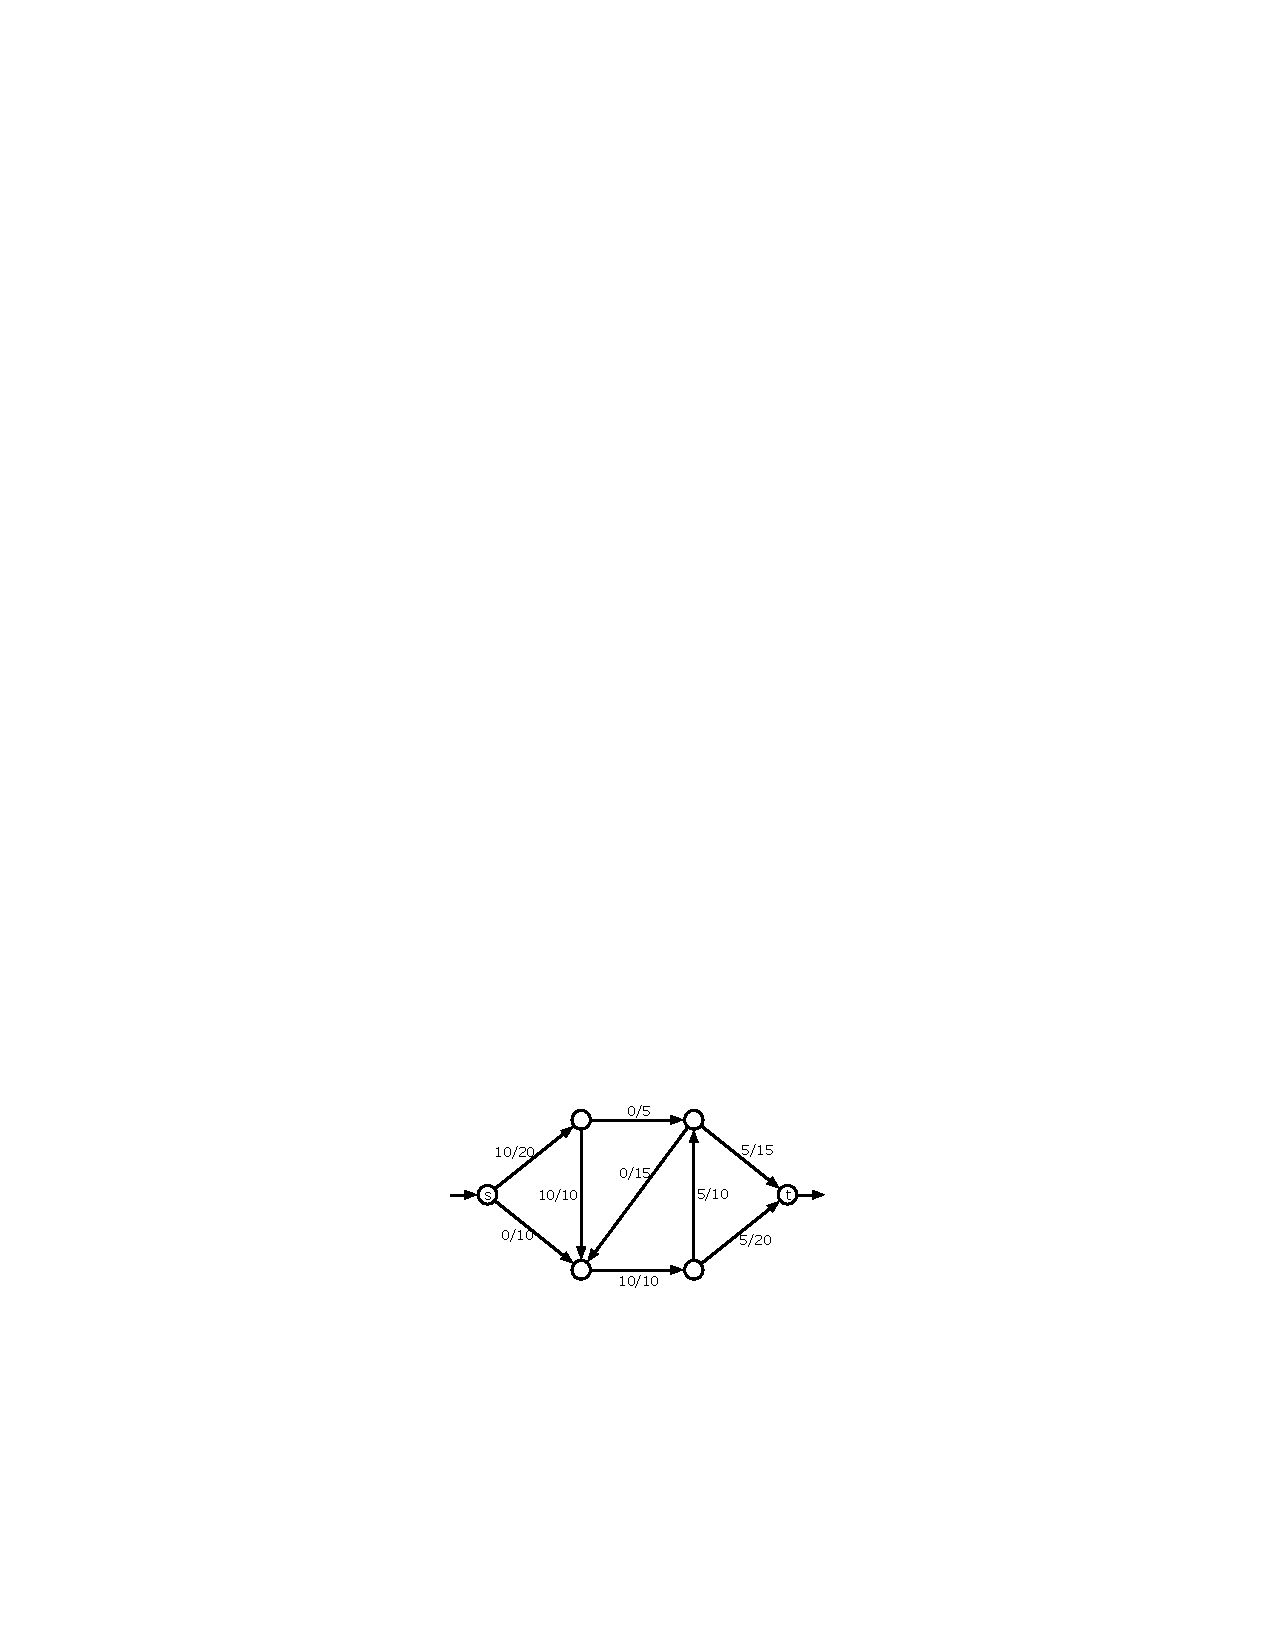
\includegraphics[scale=1.5]{fig/flowExample}
    \caption{An $(s,t)-flow$ with value 10. Each edge is labeled with its flow/capacity.}
    \label{fig:flowExample}
\end{figure}

\subsubsection{Cuts}
An $(s,t)-cut$ is a vertex bi-partition $S,T$,
i.e. $S \cap T = \emptyset$ and $S \cup T = V$, s.t. $s \in S$ and $t \in T$.

The capacity of a cut is the sum of capacities of edges
starting in $S$ and ending in $T$
\[ \|S,T\| = \sum_{v \in S}\sum_{w \in T} c(v \rightarrow w)\]

The min cut problem is to \emph{find cut whos capacity is as small as possible.}
\begin{figure}[H]
    \centering
    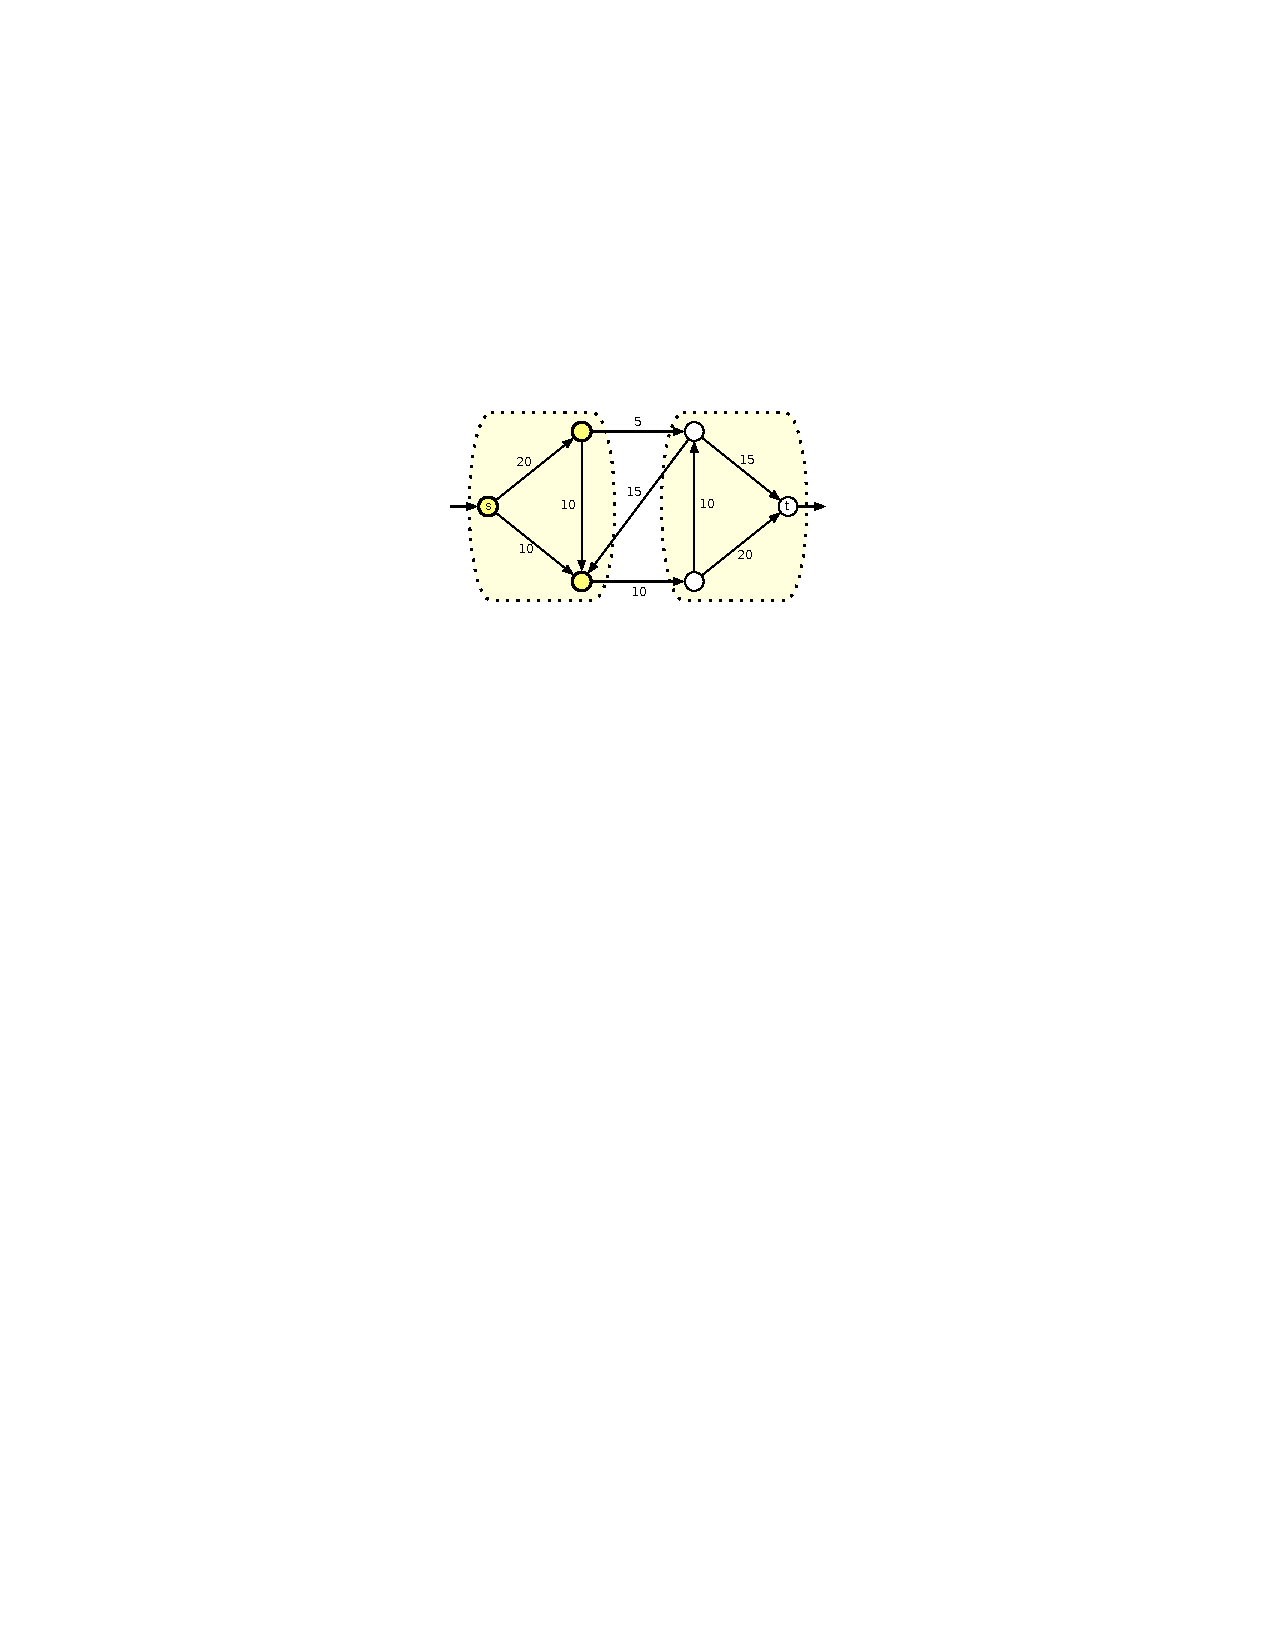
\includegraphics[scale=1.5]{fig/cutExample}
    \caption{An $(s,t)-cut$ with capacity 15. Each edge is labeled with its capacity.}
    \label{fig:cutExample}
\end{figure}

Intuitively, for any feasible $(s,t)-flow$ and any $(s,t)-cut$,
$|f| \leq \|S,T\|$. The proof is as follow:
\begin{align*}
    |f| &= \sum_w f(s \rightarrow w) - \sum_u f(u \rightarrow s) &&\text{by definition}\\
        &= \sum_{v \in S} \left(\sum_w f(v \rightarrow w) - \sum_u f(u \rightarrow v)\right) && \text{by the conservation constraint}\\
        &= \sum_{v \in S} \left(\sum_{w \in T} f(v \rightarrow w) - \sum_{u \in T} f(u \rightarrow v)\right) && \text{removing duplicate edges}\\
        &\leq \sum_{v \in S}\sum_{w \in T} f(v \rightarrow w) && \text{since $f(u \rightarrow v) \geq 0$} \\
        &\leq \sum_{v \in S}\sum_{w \in T} c(v \rightarrow w) && \text{since $f(u \rightarrow v) \leq c(u \rightarrow v)$} \\
        &= \|S,T\| && \text{by definition}
\end{align*}

\observation

$|f| = \|S,T\|$ if and only if:
\begin{itemize}
    \item $f$ avoids every edge from $T$ to $S$;
    \item $f$ saturates every edge from $S$ to $T$.
\end{itemize}

If $|f| = \|S,T\|$, then  $f$ is a max flow and $S,T$ is a min cut.
A max flow saturates all min cuts simultaneously.

\subsubsection{The Maxflow MinCut Theorem}
\begin{theorem}[The Maxflow Mincut Theorem]
    In any flow network with source $s$ and target $t$,
    the value of the maximum $(s,t)-flow$ is equal to
    the capacity of the minimum $(s,t)-cut$.
\end{theorem}

\begin{proof}

To make proof easier, assume capacity function is reduced,
i.e. for $v,w \in V$, either $c(u \rightarrow v) = 0$ or $c(v \rightarrow u) = 0$
(only one of the edges exist). This assumption is easy to enforce,
see \cref{fig:onedirection}.
\begin{figure}[H]
    \centering
    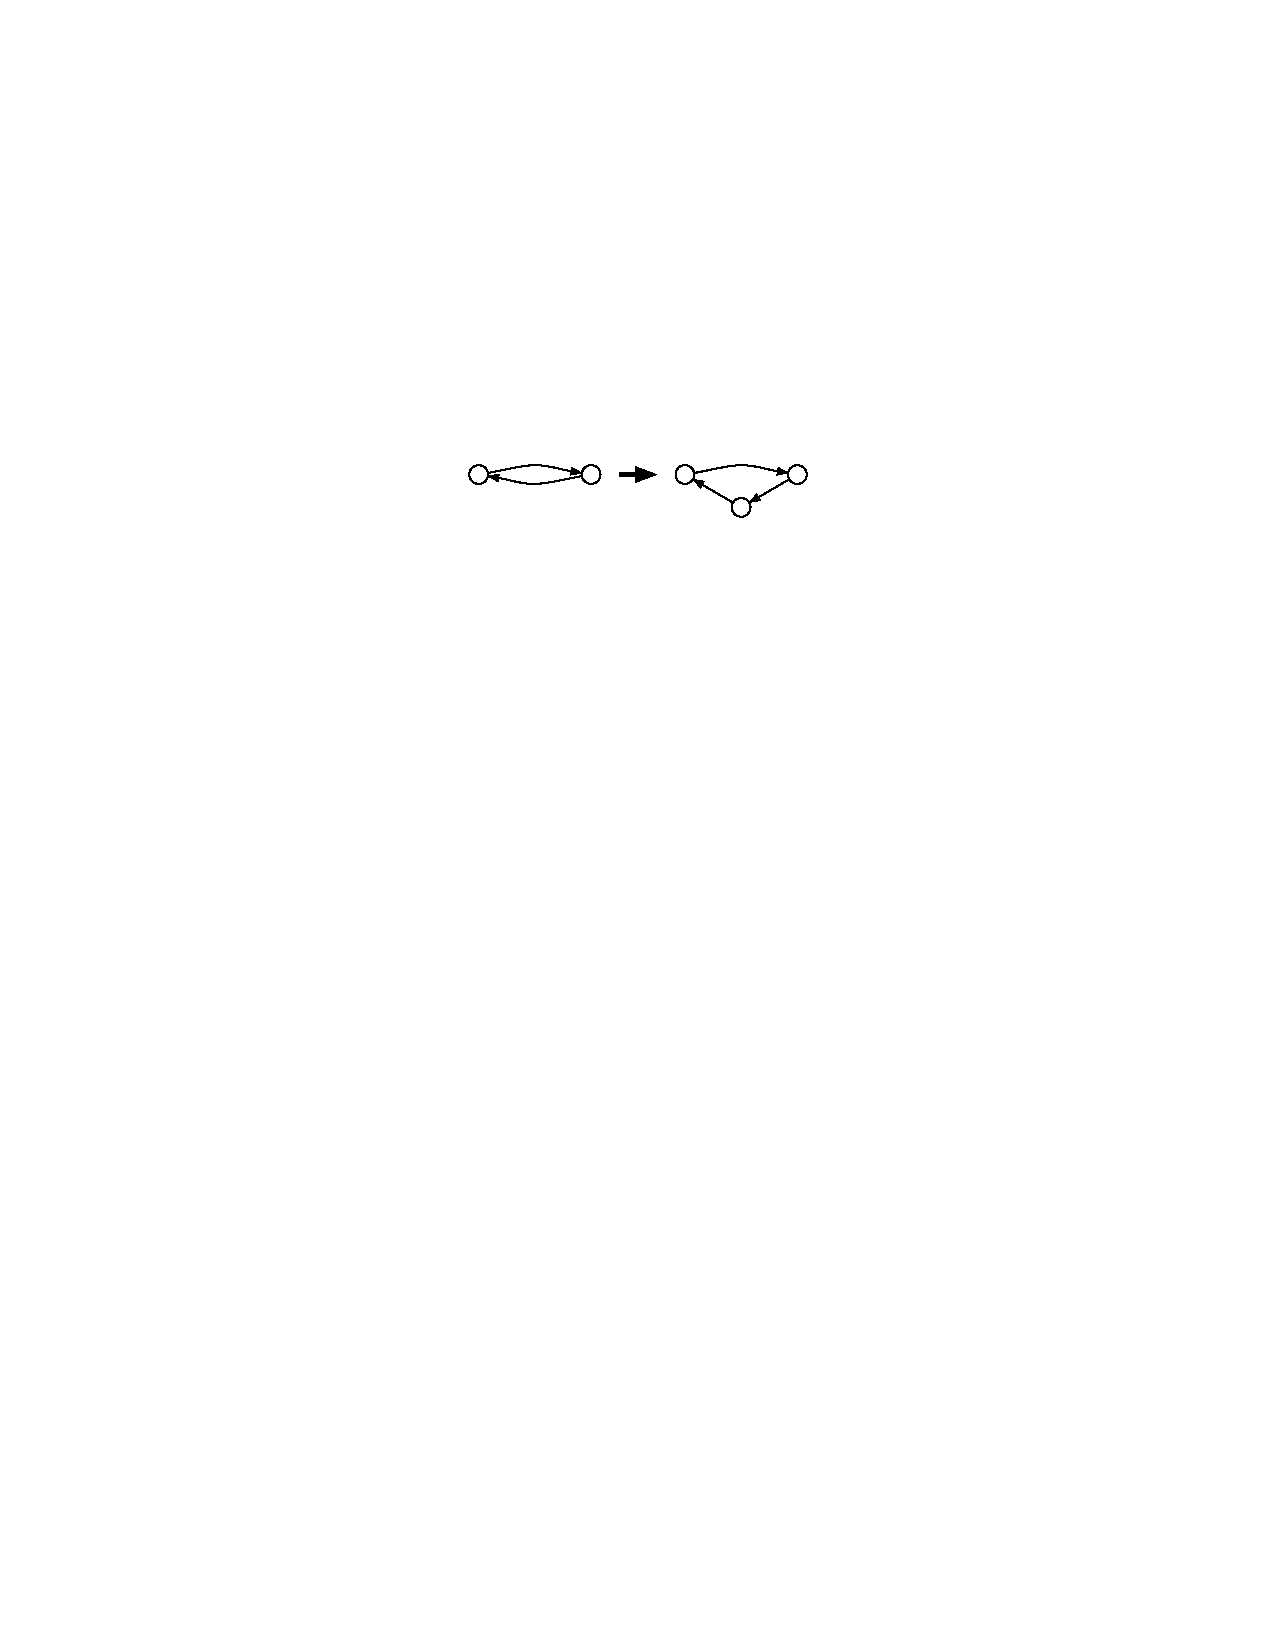
\includegraphics[scale=1.5]{fig/onedirectionassumption}
    \caption{Enforcing the one-direction assumption}
    \label{fig:onedirection}
\end{figure}

Let $f$ be any feasible flow. Define a new capacity function
$c_f:V \times V \rightarrow \mathbb{R}$, called the residual capacity,
as follows:
\begin{equation}
    c_f(u \rightarrow v) = \begin{cases}
        c(u \rightarrow v) - f(u \rightarrow v) & \text{ if } u \rightarrow v \in E\\
        f(v \rightarrow u) & \text{ if } v \rightarrow u \in E\\
        0 & \text{ otherwise } \\
        \end{cases}
\end{equation}
because edge is reduced, an pair can only in one situation.

Since $f \geq 0$ and $f \leq c$, the residual capacities are always non-negative.
Note that, we can have $c_f(u \rightarrow v) > 0$, for $u \rightarrow v \notin E$.
Thus, define residual graph as $G_f = (V, E_f)$,
where $E_f$ is the set of edges with positive residual capacity.
Notice that the residual capacities are not necessarily reduced,
it can have both $c_f(u \rightarrow v) > 0$ and $c_f(v \rightarrow u) > 0$,
as shown in \cref{fig:residualGraphExample}
\begin{figure}[H]
    \centering
    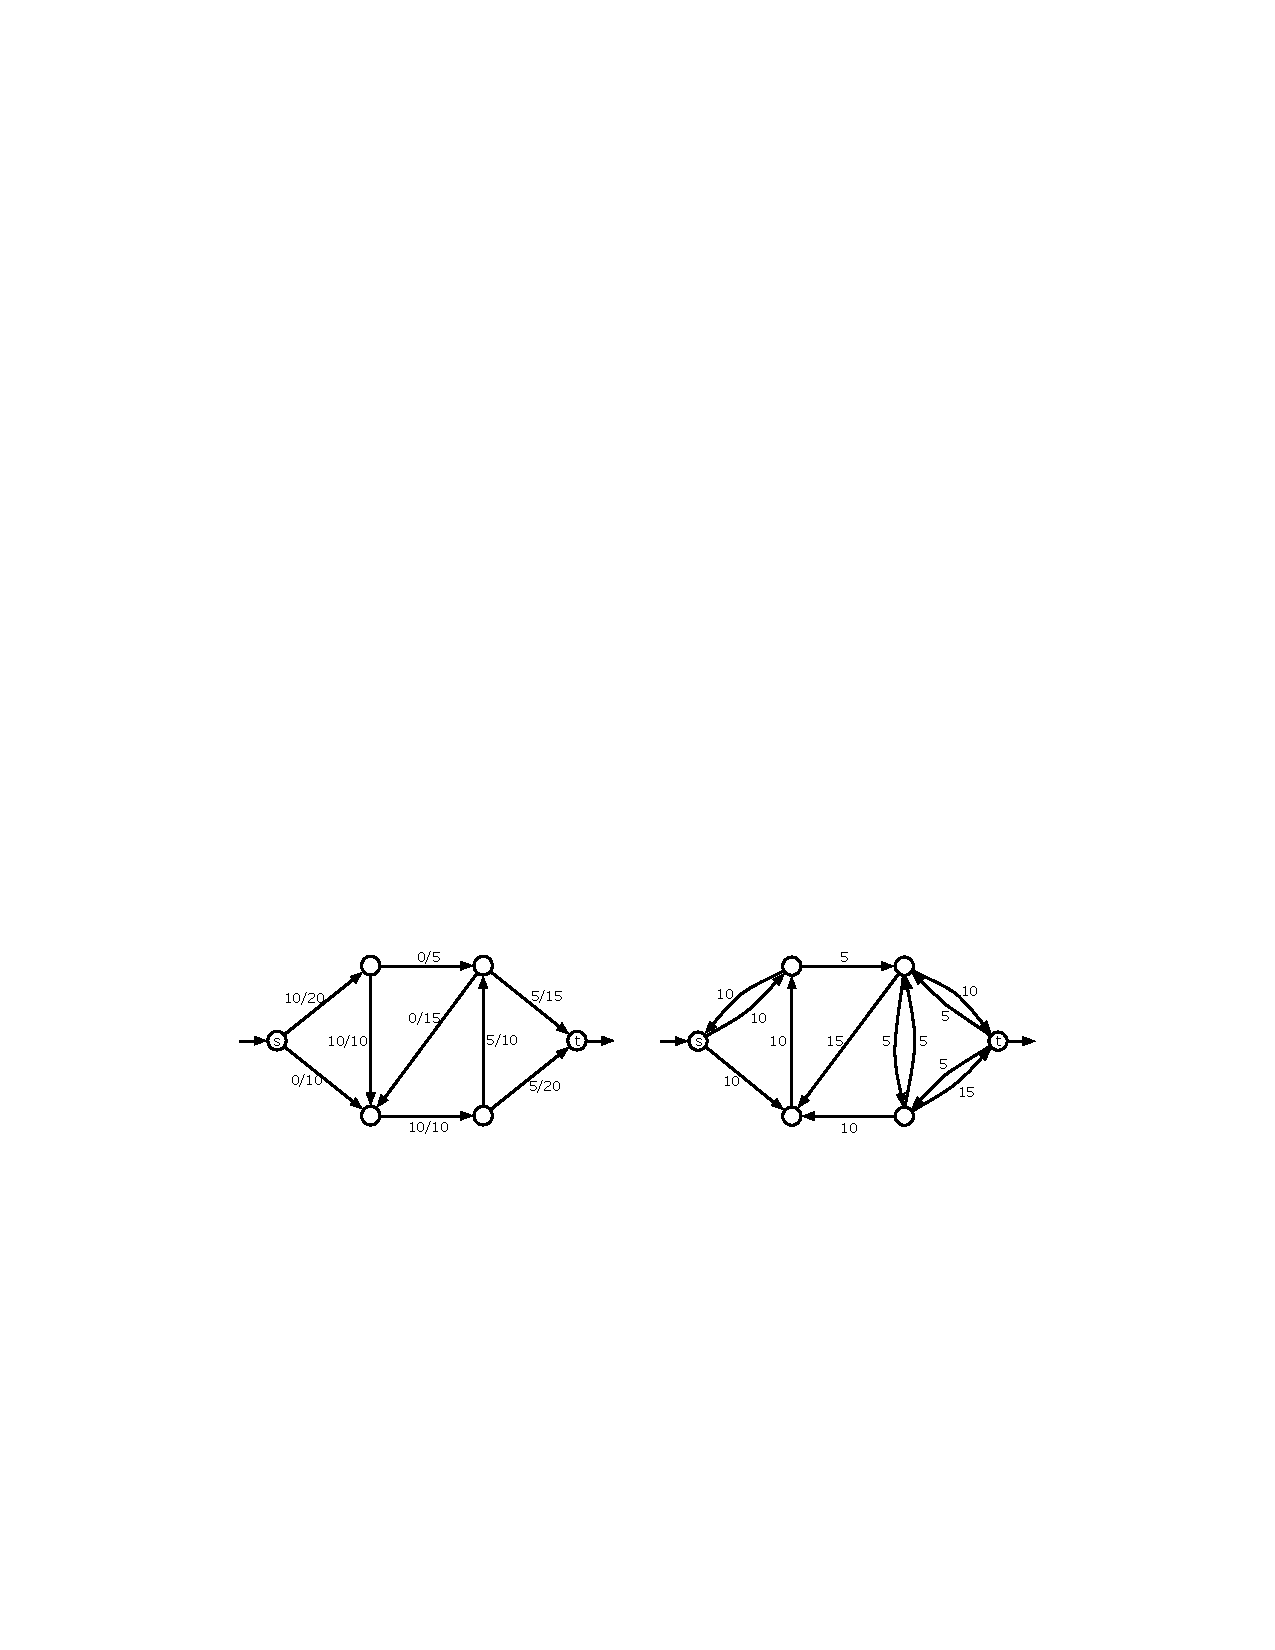
\includegraphics[width=.9\textwidth]{fig/residualGraphExample}
    \caption{A flow $f$ in a weighted graph $G$ and the corresponding residual graph $G_f$.}
    \label{fig:residualGraphExample}
\end{figure}

\begin{enumerate}[label={Case \arabic*}, leftmargin=1in]
    \item There is no path from $s$ to $t$.\\
        Let $S$ be the vertices reachable from $s$ in $G_f$,
        and let $T = V \setminus S$. \\
        Then $(S,T)$ is clearly a cut.\\
        For any $u \in S$ and $v \in T$, we have 
        \[c_f(u \rightarrow v) = (c(u \rightarrow v) - f(u \rightarrow v)) + f(v \rightarrow u) =  0 \text{ , }\]
        \begin{itemize}
            \item If $u \rightarrow v \in E$, then $c(u \rightarrow v) = 0$, i.e. saturated.
            \item if $v \rightarrow u \in E$, then $f(v \rightarrow u) = 0$, i,e, avoided.
        \end{itemize}
        So $f$ avoids every edge from $T$ to $S$ and saturates all edges from $S$ to $T$.\\
        Hence, $|f| = \|S,T\| \Rightarrow f \text{ is max flow, } S,T \text{ is min cut. }$
    \item There is a path $s = v_0 \rightarrow v_1 \rightarrow \cdots \rightarrow v_r = t$ in $G_f$.\\
        Refer to such path as an augmenting path.
        Let $F = \min_i c_f(v_i \rightarrow v_{i+1})$ denote the maximum
        amount can pass through this augmenting path.
        Define a new flow function $f^\prime:E \rightarrow \mathbb{R}$ as follows:
        \begin{equation}
            f^\prime(u \rightarrow v) =
            \begin{cases}
                f(u \rightarrow v) + F & \text{ if } u \rightarrow v \text{ is in the augmenting path } \\
                f(u \rightarrow v) - F & \text{ if } v \rightarrow u \text{ is in the augmenting path } \\
                f(u \rightarrow v) & \text{ otherwise }
            \end{cases}
        \end{equation}
        To prove that the flow $f^\prime$ is feasible with respect to original capacities $c$,
        we need to verify that $f^\prime \geq 0$ and $f^\prime \leq c$ for all edges.
\end{enumerate}
\end{proof}

